\documentclass{beamer}
\usepackage[utf8]{inputenc}
\usepackage{bookmark}
\usepackage{svg}

\usepackage{amsmath,amsthm,amssymb}
\usepackage{graphicx}% Include figure files
\usepackage{dcolumn}% Align table columns on decimal point
\usepackage{bm}% bold math
\usepackage{color}
\usepackage{epsfig}
\usepackage{multirow}
\usepackage{mathrsfs}
\usepackage{hyperref}
\usepackage{cleveref}
\usepackage{epstopdf}
\usepackage{subcaption}
\usepackage{autobreak}
\usepackage{tikz}
\usepackage{svg}

\newcommand{\V}[1]{\boldsymbol{#1}} %# vector
\newcommand{\M}[1]{\boldsymbol{#1}} %# matrix
\newcommand{\Set}[1]{\mathbb{#1}} %# set
\newcommand{\D}[1]{\Delta#1} %# \D{t} for time step size
\renewcommand{\d}[1]{\delta#1} %# \d{t} for small increment
\newcommand{\norm}[1]{\left\Vert #1\right\Vert } % norm
\newcommand{\abs}[1]{\left|#1\right|} %abs

\newcommand{\grad}{\M{\nabla}} %gradient
\newcommand{\av}[1]{\left\langle #1\right\rangle } %take average

\newcommand{\sM}[1]{\M{\mathcal{#1}}} %matrix in mathcal font
\newcommand{\dprime}{\prime\prime} % double prime
%\global\long\def\i{\iota}
%\renewcommand{\i}{\iota} %i for imaginary unit
%\renewcommand{\i}{\mathsf i} %i for imaginary unit
\newcommand{\follows}{\quad\Rightarrow\quad} %=>
\newcommand{\eqd}{\overset{d}{=}} %=^d
\newcommand{\spe}[1]{\mathscr{#1}}  %important quantities in mathscr font
\newcommand{\eps}{\epsilon}
\newcommand{\bra}[1]{\left\langle #1 \right|}
\newcommand{\ket}[1]{\left| #1 \right\rangle}
\newcommand{\braket}[2]{\left\langle #1 \middle| #2 \right\rangle}
\newcommand{\bracket}[3]{\left\langle #1 \middle| #2 \middle| #3 \right\rangle}

\title{A Poisson Solver for Dielectric Mismatches and Edge/Corner Singularities}
\date{December 11, 2025}
\author{\textbf{Xuanzhao Gao}}
% \institute{\inst{1} Center for Your Center, Flatiron Institute, Simons Foundation \and \inst{2} Other Author's Institute}

\usetheme{CCM}

\begin{document}

\begin{frame}
	\titlepage
\end{frame}

\begin{frame}
	\frametitle{Problem Formulation}
	
    An illustration of the system to be solved is shown in Fig.~\ref{fig:box3d}, where the system we are interested in is the blue region, and the yellow and gray regions are dielectric materials with different permittivities.

    \begin{figure}[htbp]
        \centering
        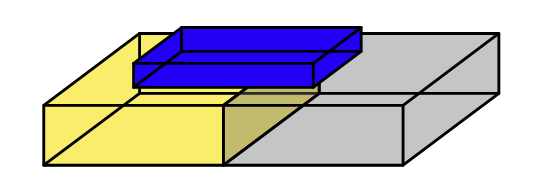
\includegraphics[width=0.4\linewidth]{figs/box3d.png}
        \caption{Illustration of the system: the bule is the material region~$\Omega_m$, the yellow and gray regions are dielectric materials:~$\Omega_1$ and~$\Omega_2$, respectively, non-filled regions are vacuum denoted as~$\Omega_0$.}
        \label{fig:box3d}
    \end{figure}

\end{frame}

\begin{frame}
	\frametitle{Problem Formulation}

    The model can be plotted in 2D space as follows, where~$\rho(x)$ is the density distribution and~$\mathbf{n}$ is the normal direction.
	\begin{figure}[htbp]
        \centering
        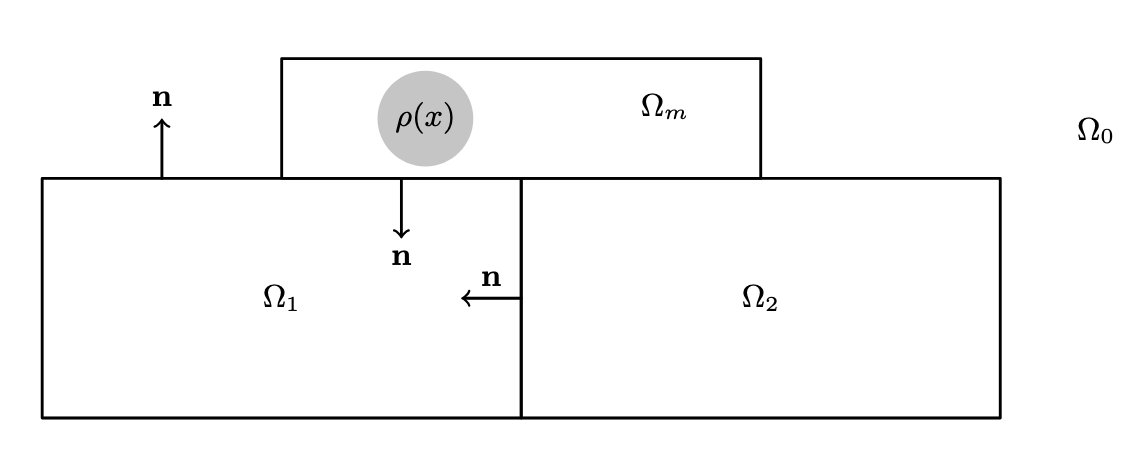
\includegraphics[width=0.6\linewidth]{figs/box2d.png}
        \label{fig:box2d}
    \end{figure}

    The dielectric permittivity is defined as a function of position:
    \begin{equation}
        \epsilon(x) = \begin{cases}
            \epsilon_m, & x \in \Omega_m \\
            \epsilon_1, & x \in \Omega_1 \\
            \epsilon_2, & x \in \Omega_2 \\
            \epsilon_0 = 1, & x \in \Omega_0
        \end{cases}
    \end{equation}

\end{frame}

\begin{frame}
	\frametitle{Problem Formulation}

    The potential~$\phi(x)$ can be represented as the solution to the Poisson equation:
    \begin{equation}\label{eq:poisson-origin}
        \grad_{x} \cdot \left( \epsilon(x) \grad_{x} \phi(x) \right) = - \rho(x),
    \end{equation}
    which can be rewritten as the following boundary value problem (indices omitted for simplicity):
    \begin{equation}
        \begin{cases}
            \epsilon_m \Delta_{x} \phi(x) = - \rho(x)~, & x \in \Omega_m \\
            \Delta_{x} \phi(x) = 0~, & x \in \Omega_0 \cup \Omega_1 \cup \Omega_2 \\
            \phi(x)\mid_{\partial \Omega_i} = \phi(x)\mid_{\partial \Omega_j}~, & x \in \partial \Omega_i \cap \partial \Omega_j \\
            \epsilon_i \mathbf{n} \cdot \grad_{x} \phi(x)\mid_{\partial \Omega_i} = \epsilon_j \mathbf{n} \cdot \grad_{x} \phi(x)\mid_{\partial \Omega_j}~, & x \in \partial \Omega_i \cap \partial \Omega_j \\
            \phi(x) \to 0~, & \abs{x} \to + \infty \\
        \end{cases}
    \end{equation}
    We will show that these equations can be transformed into a boundary integral equation for the potential~$\phi(x)$ with a single layer potential~$\mathbf{\sigma}(x)$ on the boundaries.

\end{frame}

\begin{frame}
	\frametitle{Boundary Integral Equation}

	The potential~$\phi(x)$ is separated into two parts:
    \begin{equation}
        \phi(x) = u(x) + u_{\text{inc}}(x),
    \end{equation}
    where~$u(x)$ is the scattered potential, and~$u_{\text{inc}}(x)$ is the incident potential.
    The incident potential satisfies:
    \begin{equation}
        \begin{cases}
        \epsilon_m \Delta u_{\text{inc}}(x) = - \rho(x), & x \in \mathbb{R}^3 \\
        u_{\text{inc}}(x) \to 0, & \abs{x} \to + \infty 
        \end{cases}
    \end{equation}
    which is given by the following integral:
    \begin{equation}
        u_{\text{inc}}(x) = \frac{1}{4 \pi \epsilon_m} \int \frac{\rho(x')}{|x - x'|} \mathrm{d}x'\;.
    \end{equation}
    Then the scattered potential satisfies:
    \begin{equation}\label{eq:scattered-potential-boundary}
        \begin{cases}
        \Delta u(x) = 0, & x \in \Omega_i \\
        \epsilon_i \partial_{\mathbf{n}} \left( u^+(x) + u_{\text{inc}}(x) \right) = \epsilon_j \partial_{\mathbf{n}} \left( u^-(x) + u_{\text{inc}}(x) \right), & x \in \partial \Omega_i \cap \partial \Omega_j \\
        u(x) \to 0, & \abs{x} \to + \infty 
        \end{cases}
    \end{equation}
    which is a piecewise continuous function in each region.
\end{frame}

\begin{frame}
	\frametitle{Boundary Integral Equation}

    Under the single layer potential representation, the scattered potential is given by
    \begin{equation}
        u(x) = \frac{1}{4 \pi} \int_{\Gamma} \frac{\mathbf{\sigma}(x')}{|x - x'|} \mathrm{d}S(x'),
    \end{equation}
    where~$\Gamma$ is all boundaries in the system.
    Due to the existence of the single layer potential, the normal component of the scattered potential is given by
    \begin{equation}\label{eq:scattered-potential}
        \begin{split}
        \partial_{\mathbf{n}} u(\mathbf{r^+}) &= \frac{1}{4 \pi} \mathbf{n} \cdot \int \grad_{x} \frac{\mathbf{\sigma}(x')}{|x - x'|} \mathrm{d}S(x') - \frac{\sigma(x)}{2}, = D^T \mathbf{\sigma}(x) - \frac{\sigma(x)}{2} \\
        \partial_{\mathbf{n}} u(\mathbf{r^-}) &= \frac{1}{4 \pi} \mathbf{n} \cdot \int \grad_{x} \frac{\mathbf{\sigma}(x')}{|x - x'|} \mathrm{d}S(x') + \frac{\sigma(x)}{2} = D^T \mathbf{\sigma}(x) + \frac{\sigma(x)}{2},
        \end{split}
    \end{equation}
    where $D^T$ represents the integral operator $\int_{\Gamma} \grad_{x} \frac{\mathrm{d}S(x')}{|x - x'|}$.
\end{frame}

\begin{frame}
    \frametitle{Boundary Integral Equation}

    Then the first and third equations of Eq.~\eqref{eq:scattered-potential-boundary} are automatically satisfied, and the second equation can be rewritten as
    \begin{small}
        \begin{equation}
        \epsilon_i \left( D^T \mathbf{\sigma}(x) - \frac{\sigma(x)}{2} + \partial_{\mathbf{n}} u_{\text{inc}}(x) \right) = \epsilon_j \left( D^T \mathbf{\sigma}(x) + \frac{\sigma(x)}{2} + \partial_{\mathbf{n}} u_{\text{inc}}(x) \right),~x \in \partial \Omega_i \cap \partial \Omega_j.
        \end{equation}
    \end{small}
    or equivalently,
    \begin{equation}\label{eq:sl_equation}
        \frac{1}{2} \frac{\epsilon_i + \epsilon_j}{\epsilon_i - \epsilon_j} \sigma(x) + D^T \sigma(x) = - \partial_{\mathbf{n}} u_{\text{inc}}(x),~x \in \partial \Omega_i \cap \partial \Omega_j.
    \end{equation}
    The equation is a Fredholm integral equation of the second kind, and is identical to Eq.~(2.19) in Ref.~\cite{greengard1994numerical}.
\end{frame}

\begin{frame}
    \frametitle{Boxes in 2D}

    We first consider boxes in 2D space, the results are shown as follows:
    \begin{figure}[htbp]
        \centering
        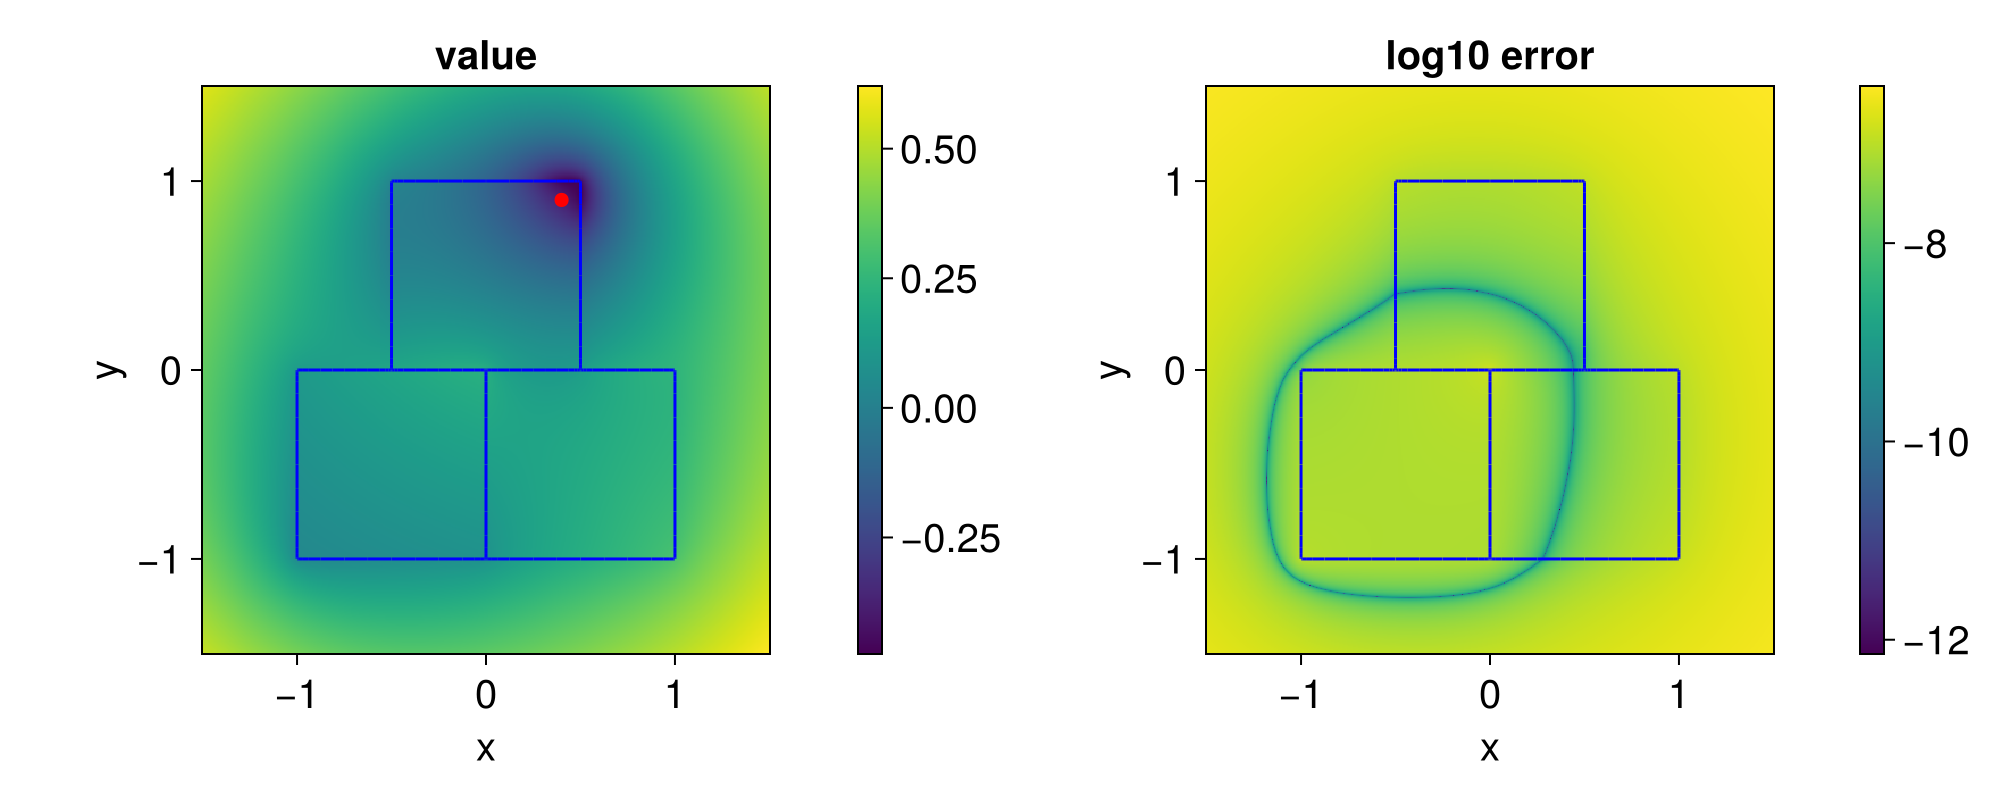
\includegraphics[width=0.8\linewidth]{../codes/box2d/figs/mbox_fmm2d_3.png}
        \caption{Contour plots of the potential~$\phi(x)$ and the error, where the reference solution is generated by ~$30$ adaptations: $\epsilon_1 = 100.0$, $\epsilon_2 = 3.0$, and $\epsilon_m = 4.0$.}
    \end{figure}

\end{frame}

\begin{frame}
    \frametitle{Boxes in 2D}

    Convergence of the method to order of the quadrature and number of adaptations are shown as follows: (left) error decay for different values of quadrature points in each panel, with number of adaptations fixed to 20. (right) error decay for different values of number of adaptations, with quadrature points fixed to 16 in each panel.
    \begin{figure}[htbp]
        \centering
        \includesvg[width=0.9\linewidth]{../codes/box2d/figs/convergence_mbox.svg}
        \caption{Convergence of the single layer potential on the boundaries with adaptive discretization for multiple boxes.}
        \label{fig:2d-multiple-boxes-convergence}
    \end{figure}

\end{frame}

\begin{frame}
    \frametitle{Boxes in 2D}

    Condition number of the linear system and number of iterations for GMRES solver to converge to the solution are shown in Fig.~\ref{fig:2d-multiple-boxes-condition-number}.
    Since the largest eigenvalue is exactly~$0.5$, thus the problem defined by Eq.~\eqref{eq:sl_equation} is ill-conditioned when $\epsilon_m \to \infty$.

    \begin{figure}[htbp]
        \centering
        \includesvg[width=0.8\linewidth]{../codes/box2d/figs/condition_number.svg}
        \caption{Condition number of the linear system for different values of ~$\epsilon_m$ and number of iterations for GMRES solver to converge to the solution.}
        \label{fig:2d-multiple-boxes-condition-number}
    \end{figure}

\end{frame}

\begin{frame}
    \frametitle{Divergence of the single layer density near the corner}

    We find that the single layer density near the corner diverges in speed of
    \begin{equation}
        \sigma(x) = O \left( x^{k} \right)\;,
    \end{equation}
    where~$k$ is dependent on the value of~$\gamma$.
    Specifically, when~$\gamma = \pm 1$, i.e. $\epsilon_m = \infty$ or $0$, ~$k = -1/3$.
    A theoretical solution is also shown in the right panel, consistent with the theory in Ref.~\cite{van2007electromagnetic}.
    
    \begin{figure}[htbp]
        \centering
        \begin{subfigure}[c]{0.58\linewidth}
            \centering
            \includesvg[width=\linewidth]{../codes/box2d/figs/blowup_rate.svg}
            % \caption{Fitted blowup rate $k$ for different values of~$\gamma$.}
            % \label{fig:2d-box-k}
        \end{subfigure}
        \hfill
        \begin{subfigure}[c]{0.4\linewidth}
            \centering
            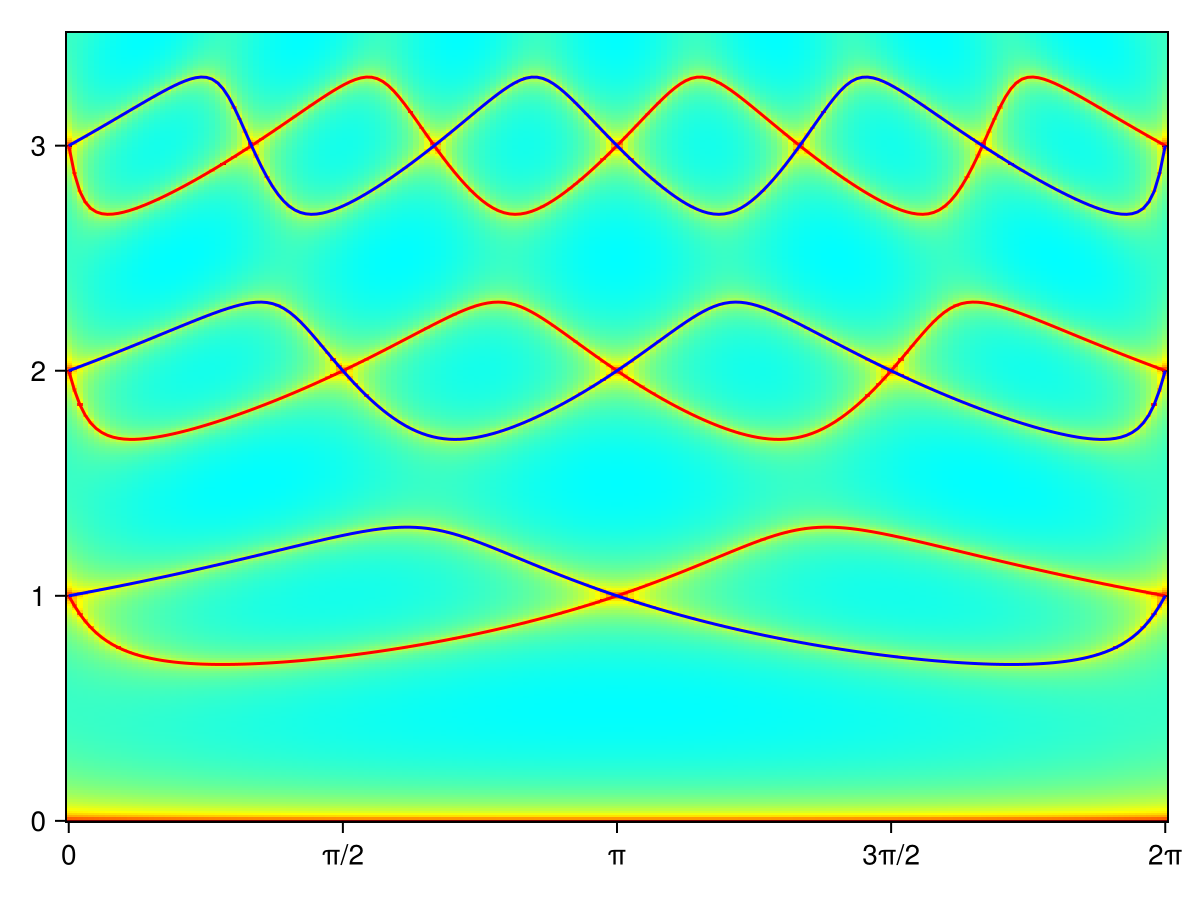
\includegraphics[width=\linewidth]{../codes/box2d/figs/blowup_rate_compare.png}
            % \caption{Spectrum of the blowup rate $k$ for different values of~$\gamma$.}
            % \label{fig:2d-box-blowup-spectrum}
        \end{subfigure}
        \caption{(Left) Fitted blowup rate $k$ for different values of~$\gamma$. (Right) Spectrum of the blowup rate $k + 1$ for different values of~$\gamma$.}
        \label{fig:2d-box-blowup-analysis}
    \end{figure}
    
\end{frame}

\begin{frame}
    \frametitle{Box in 3D}

    For box in 3D, we consider the following discretization strategies:
    (a) non-adaptive discretization with a large number of quadrature points,
    (b) adaptive discretization with fixed number of quadrature points,
    (c) adaptive discretization with gradually reduced number of quadrature points.

    \begin{figure}[htbp]
        \centering
        \begin{subfigure}[b]{0.3\textwidth}
            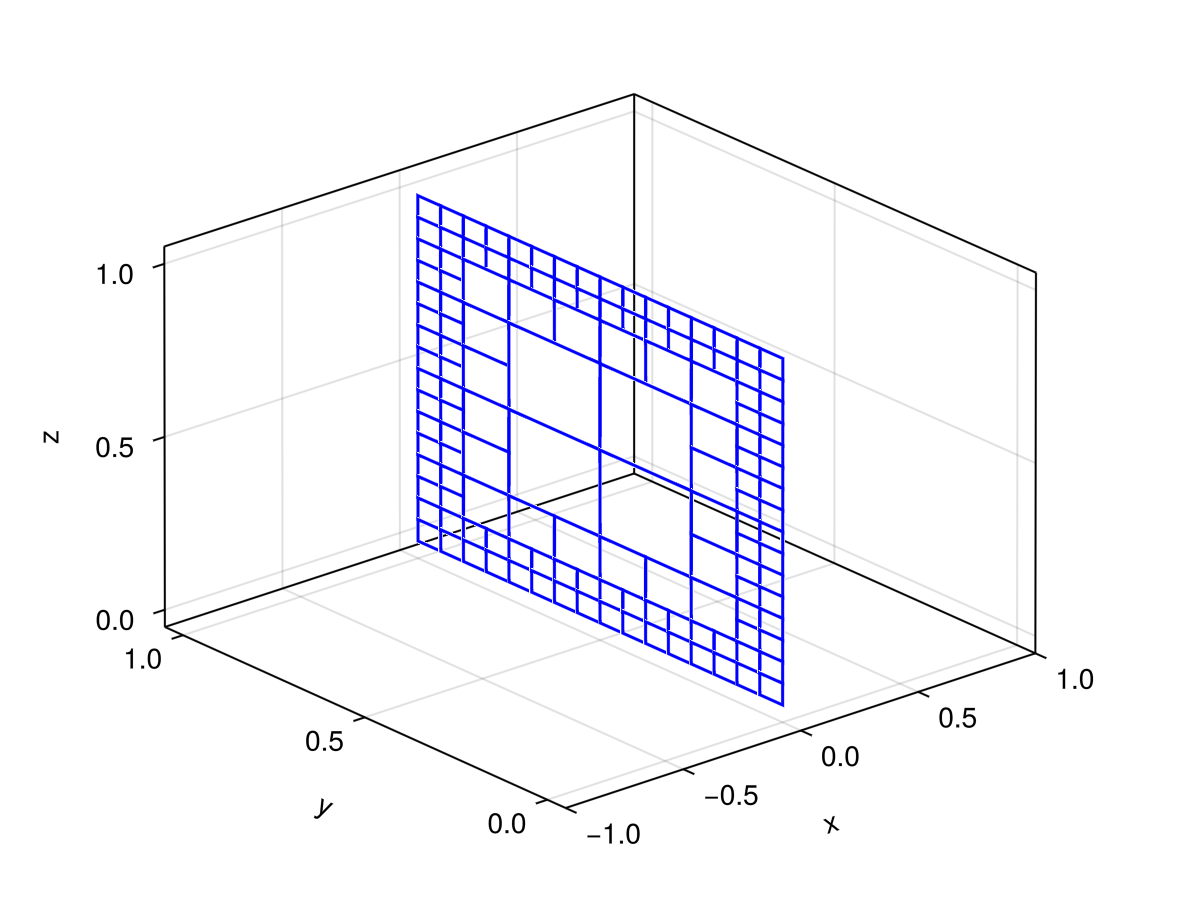
\includegraphics[width=\linewidth]{figs/squares.png}
        \end{subfigure}
        \begin{subfigure}[b]{0.3\textwidth}
            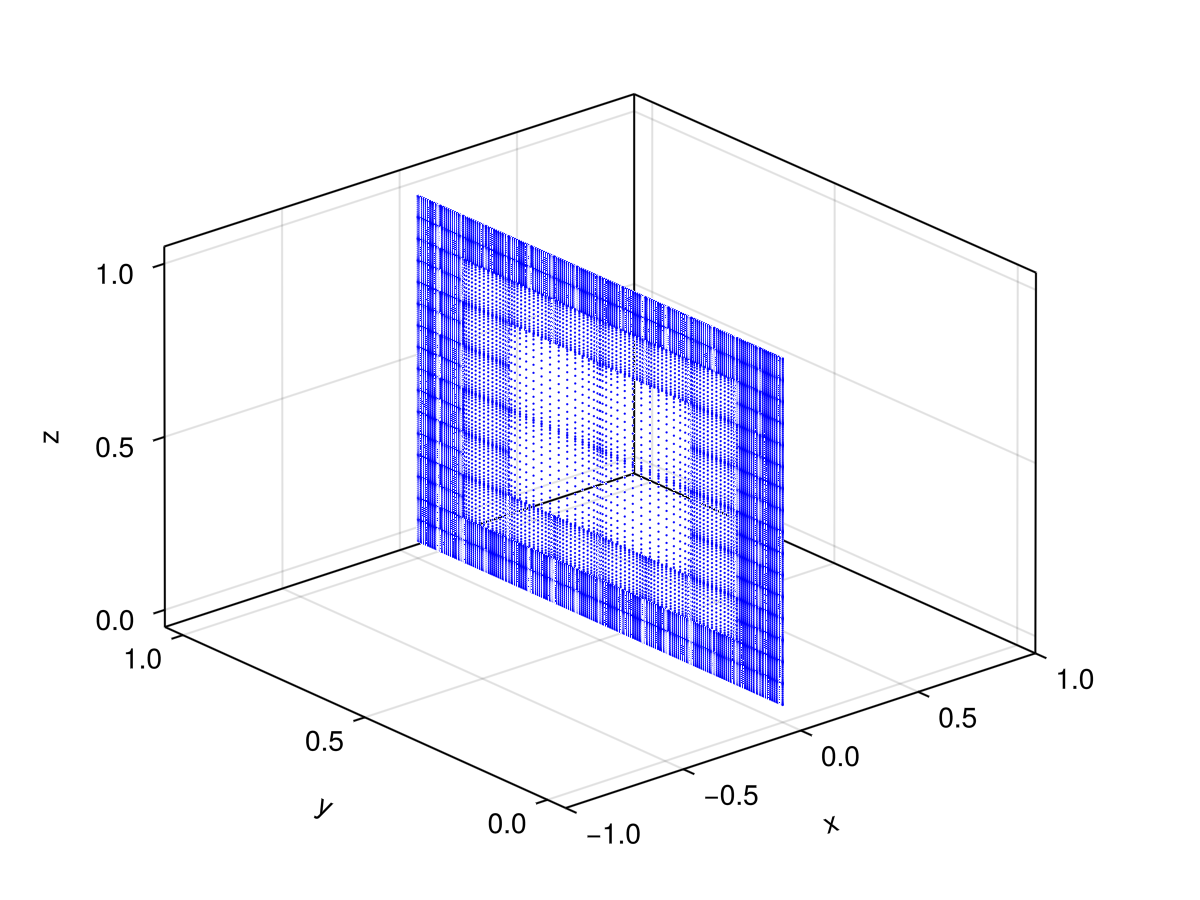
\includegraphics[width=\linewidth]{figs/discretization.png}
        \end{subfigure}
        \begin{subfigure}[b]{0.3\textwidth}
            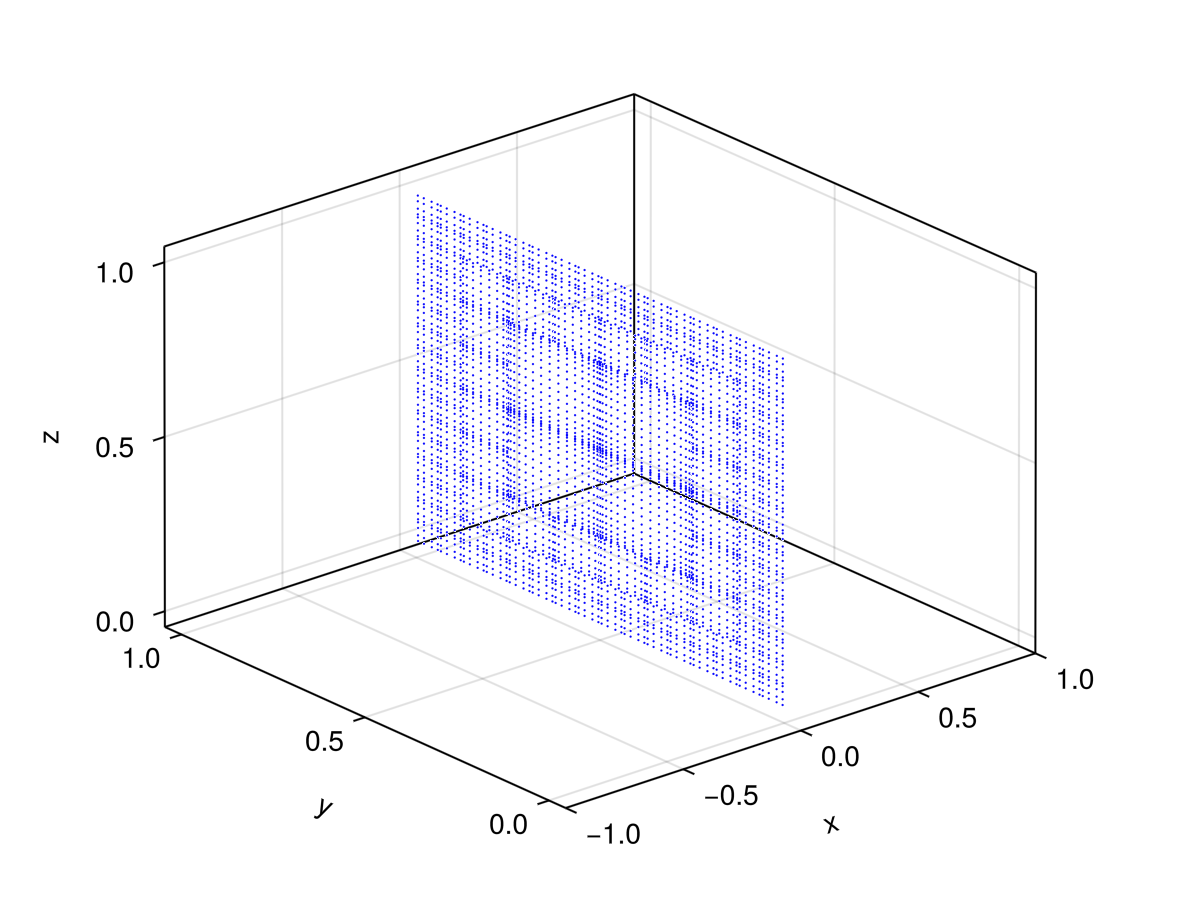
\includegraphics[width=\linewidth]{figs/reduced_discretization.png}
        \end{subfigure}
        \caption{Discretization of the surfaces in 3D: (a) the panels, (b) the quadrature points is fixed on the panels, (c) the quadrature points is gradually reduced when the panel is close to the edges and corners.}
        \label{fig:3d-box-discretization}
    \end{figure}

\end{frame}

% \begin{frame}
%     \frametitle{Box in 3D}
    
%     We first check the Green's identity for the double layer operator, i.e. $D 1 = - \frac{1}{2}$.

%     \begin{figure}[htbp]
%         \centering
%         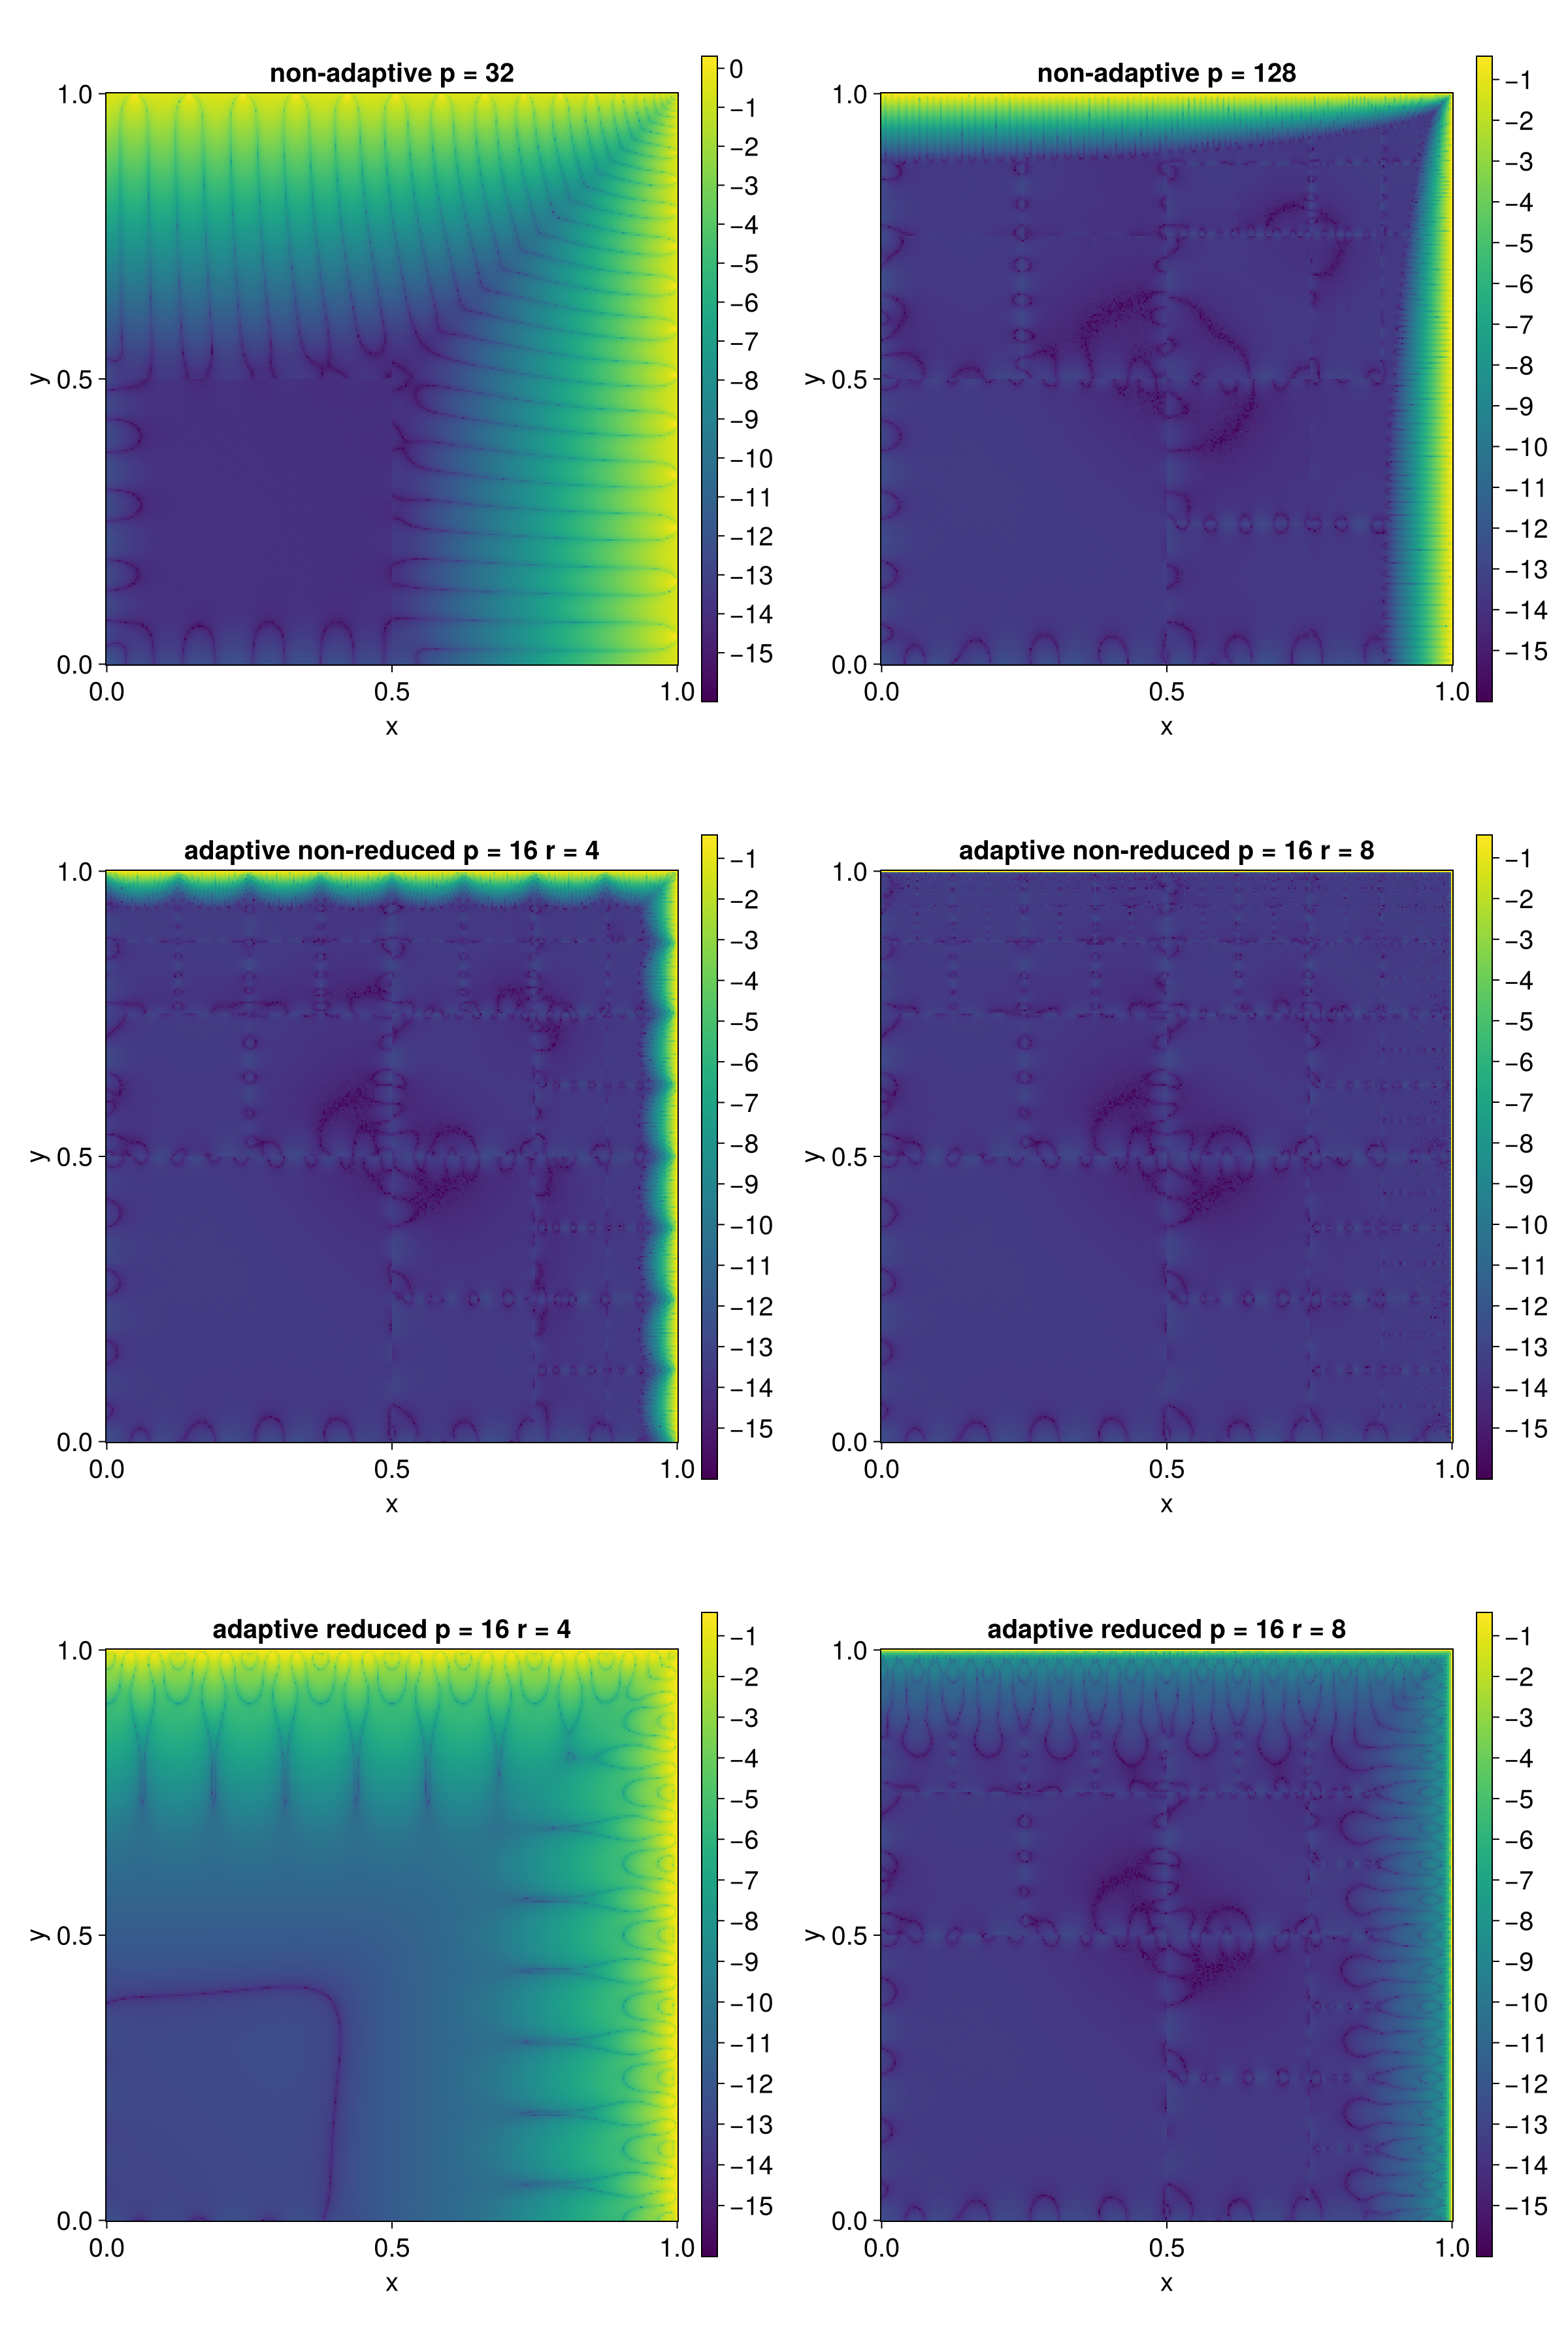
\includegraphics[width=0.4\linewidth]{../codes/box3d/figs/single_box3d_gi_heatmap.png}
%         \caption{Error of the Green's identity for different discretization strategies. The first row are non-adaptive discretization (notice that the lines are because FMM3D is used for evaluation), the second row are adaptive discretization with fixed number of quadrature points, the third row are adaptive discretization with gradually reduced number of quadrature points. $p$ is the order of the quadrature, $r$ is number of adaptations.}
%         \label{fig:3d-box-green-identity}
%     \end{figure}
    
% \end{frame}

\bibliography{ref}
\bibliographystyle{plain}

\end{document}
